This dissertation shows ways to provide autonomous feedback for a range of assignment types in online computer science education. I believe that the ideas presented in this thesis are a step towards inclusive, quality education at scale.

\section{A New Grand Challenge}

The nascent field of computational education, sits at the confluence of a great need and a new hope that progress should be possible. While the problems of education are thousands of years old the emergence of massive online datasets of students learning and a synchronous evolution in machine learning has allowed us to revisit many deep and old problems. 

The foremost problem in computational education -- both because of its potential for impact and because of its applicability for data driven solutions -- is the question: How can we develop a learner model that is both convincing in its ability to make predictions and useful for helping students achieve their learning objectives? The magnitude of the intellectual merit and societal impact involved in answering this question make this question worthy of being a grand research challenges.

\section{The Shortage of Quality Education}

To put it simply there is great need to increase the productivity of education.

In the end of the year 2000, at the edge of the East River in New York City, the largest gathering of world leaders convened for the Millennial Summit to seize the compelling symbolism of a unique moment in time and reflect on the future the leaders hoped for. At the meeting, the delegates came to the consensus that increasing education should be one of the primary foci of humankind. They declared that it was, ``a foundation for human fulfillment, peace, sustainable development, economic
growth, decent work, gender equality and responsible global citizenship." In the summit the delegates encoded their desiderata for the future into a set of twelve Millennium Development Goals to be achieved by December 31\ts{st} 2015. One of the concrete goals was to attain universal primary education. 

We are a month away from the Millennium Development Goals deadline. As such, it a particularly interesting point in time to reflect on where the world stands with respect to providing education. In the words of the United Nations, the education Millenium Development Goal of universal primary education will be ``unifinished." The global primary completion rate has reached 90\%\footnote{Net completion rate is the ratio of children of official school age who have completed a course to the population of the corresponding official school age. Secondary education completes the provision of basic education that began at the primary level, and aims at laying the foundations for lifelong learning and human development, by offering more subject- or skill-oriented instruction using more specialized teachers.} (according to the world bank) and the secondary and tertiary \emph{enrollment} rates are around 60\% and 20\% respectively \cite{world2015world}. The most palpable meaning hidden behind these statistics is the sheer magnitude of human potential around the world that is being lost. Hundreds of millions of people don't have the opportunity to even enroll in secondary school. Looking even slightly deeper into the impact of the Millenium Development Goal further highlights the magnitude of the education challenge. Many who enroll don't complete, and completion does not mean that students are proficient with respect to the desired learning outcomes. Quality, it seems was an essential word left out of the initial objective. There are many different ways in which you could experience primary school, and in the attempt to provide primary school for all, it is not desirable to have to produce a worse experience. Even when quality cannot be fully captured by metrics it should be a core part of the education conversation.

This year the Millennium Development Goals will be replaced by the United Nations Sustainable Development Goals. The new education objective is to, ``Ensure inclusive and quality education for all and promote lifelong learning." It includes subgoals for universal access to both primary and secondary education with expanded channels for tertiary and adult education opportunities. The deadline to meet this new goal is 2030. 
To me this high bar makes sense: inclusive high quality education. Lack of access to education is a great injustice and the sooner we address it, the sooner we can reap the rewards of a more equal world. But the magnitude of the equal access to quality education challenge is titanic. 

I am absolutely in favor of the most obvious way forward: we could allocate the necessary resources to train and hire enough teachers to achieve high quality accessible education using the same hundred year old formula. Though as shown by the limited success of the Millennium Development Goals, it is not a panacea. There are a few shortcomings to this strategy. Quality education at scale is expensive. The average OECD nation spent \$9,313 per young person \cite{oecd2014education} and the most optimistic estimates for the cost of the Sustainable Development Goals is on the order of US\$239 billion. The cost can be taken on by governments, aid donations or individually. Based on the inability to achieve the Millennium Development Goal it seems there is not enough political will to foot the necessary cost, and there is appreciable fear of aid dependency on the part of developing nations. 

The problems run deeper than lack of political will. In his lecture series The Cost Disease of Education, William Bowen makes the observation that the cost per student of education is rising appreciably faster than an economy-wide index of costs in general \cite{bowen2012cost}. As he concludes, ``The consistency of this pattern suggested to me then, as it does today, that we are observing the effects of relationships that are deeply embedded in the economic order." He then goes on to explain, ``The basic idea is simple: in labor-intensive industries such as
the performing arts and education, there is less opportunity than in other sectors
to increase productivity by, for example, substituting capital for labor. Yet, over
time, markets dictate that wages for comparably qualified individuals have to
increase at roughly the same rate in all industries. As a result, unit labor costs
must be expected to rise relatively faster in the performing arts and education
than in the economy overall." The cost of education is already too high and yet it is predicted to increase. In the United States one side effect of the cost is that private education debt held by students is now \$1.2 trillion and has surpassed consumer debt. 

So how do we move forward? A complementary way to help make progress towards the goal of equal access to quality education is to increase educational productivity. It is also the theoretical solution to the cost disease. The productivity ratio is a high level representation of how much educational utility that we get out per unit of effort we put in. 
\begin{align*}
\text{Productivity} &= \text{Educational Output / Unit of Input} 
\end{align*}
And it can be increased by either making it easier for teachers to engender the same learning objectives, or given a fixed amount of work, allow teachers to achieve more. Increasing productivity would make the price tag of  quality education cheaper, and therefore universal education more achievable. This suggests a potential area in which a technology solution could be useful. 

The fanfare that accompanied the creation of Coursera and EdX, education platforms that promised free access to the materials of premier universities, largely built off of a recognition of the need for higher education productivity. Massive Open Access Courses (MOOCs) engendered hope that constant iterative
improvement and economies of scale of the internet could increase productivity and counter the cost disease.

\section{Feedback}

While there has been notable progress in our ability to deliver educational material, the ability to scale up the delivery of feedback to assignments that are more difficult than trivial multiple-choice questions or simple answers, has remained elusive. We define assignment feedback as both getting a grade and comments on a submitted piece of work \emph{and} providing help to learners who are stuck. These types of feedback correspond to two high level forms of assessment from education literature: Formative assessment, where the goal of an assignment is to help a student learn and summative assessment, where the goal of an assignment is to measure what a student knows.

Feedback is a cornerstone of the educational experience. It is also one of the most time consuming parts of teaching \cite{sadler2006impact}. Traditional teachers often face a trade off when they develop assignments. On one hand, they want to generate assignments that are engaging and that capture the variety of ways that course concepts can interact. On the other hand they need to accommodate limitations in resources and time. Often in classrooms, which we would anecdotally consider high quality learning experiences, teachers opt for rich assignments. The cost in teacher time is high. A study of American public school teachers in 1994 showed that teachers spent on average 19\% of their time outside of class grading and preparing assessments. This directly contributed to them being overworked. The average teacher spent 43.8 hours a week working \cite{henke1996schools}.

\begin{table}[t]
 \centering
 \ra{1.3}
 \begin{tabular}{ l l }
 \toprule
	Activity & Hours per Week \\
   \midrule
   Outside class, grading and preparring assessments & 8.5 \\
  Outside class, with students & 3.3 \\
  In class & 32.0 \\
  Total time & 43.8 \\
  \bottomrule
  \end{tabular}
  \caption[Teacher time]{How public school teachers time is spent. Based on statistics from 1994 \cite{henke1996schools}}
 \label{tab:dataTable}
\end{table}

This matches with my anecdotal experience. While the above statistics on teacher work only apply to public school teachers, the large amount of time needed to provide feedback seems ubiquitous across almost all teaching mediums. In fact, as classes increase in complexity feedback tend to becomes more laborious. In university courses assessing student work often requires highly skilled teaching assistants hundreds of hours a term.

Moreover, providing feedback, especially grading, has the tenor of being a highly repetitive task. There is a palpable sensation that when I am helping students who are stuck, or grading assignments, once I have seen enough student work I have a good idea of most ways that students will need feedback. As such it seems ideal for automation. Can we develop a technological solution to increase teacher productivity when grading? Solving this problem could substantially help towards the goal of inclusive quality education. If feedback can be personalized and instantaneous it can have benefits beyond those enjoyed in a conventional classroom. In his now famous work, the Two-Sigma Problem, Benjamin Bloom notes that on average students who are taught by a tutor with feedback-corrective procedures perform better that 98\% of students in conventional classroom \cite{corbett2001cognitive}. In addition, maybe we would not have to spend as much time testing students if we sufficiently mastered the ability to understand their work. Simply the act of learning would be enough for us to evaluate the status of each student.  

\section{Online Programming Case Study}

Online learning engendered hope. Many thought that the constant interactive improvement and economies of scale of the internet can help answer the question: How does high quality, inclusive, education scale? 
That hope gained substantial traction in 2011 when Stanford, Harvard and MIT opened up access to the materials for some of the most prestigious courses in the world for free. These online versions of university courses have been dubbed MOOC (Massive Open Online Courses). MOOCs are
structured learning environments that emphasize instructional
videos and regular assessments, centralizing activities
on a single platform. They exist for six to ten weeks at a time as virtual, distributed classrooms. Tens of thousands of students began to engage in materials for courses which had previously only been accessible to a few hundred. MOOCs joined an ecosystem that had already shown the ability to tap into enormous demand such as Khan Academy, whose mission is to provide, ``a free, world-class education for anyone, anywhere" and was serving millions of students. The excitement was high and the New York Times declared the Year of the MOOC \cite{pappano2012year}. 

The internet allowed the distribution of course content to scale well. It even allowed for rich peer communication amongst learners. However, in courses where the student-teacher ratio is be ten thousand to one or worse, it has been impossible for instructors to personally give hints to students or to understand the multitude of student approaches and pitfalls. As a result online courses are faced with a trade-off. Either given rich beautiful assignments that have little to no staff feedback. Or, on the other hand give short answer questions and provide limited, rote feedback. Both options are lacking. It is hard to imagine an education that doesn't involve engaging assignments and the scaffolding and feedback for those assignments that are a staple of the in-person classroom experience. A common solution has been to use peer grading. While peer assessment has some notable benefits it does not allow for feedback to students who are stuck and it is a major increase in time commitment for students.

It is unclear the role that online education will eventually play in helping provide universal access to high quality education. Regardless, the current iteration of online platforms have produced a unique opportunity to study learning. Student work is stored electronically. As a learner works through an assignment often a digital record of their progress is saved. The courses are large, which means that we can confirm our results with higher level of confidence. What we learn from these environments we believe will translate more broadly. Hopefully we can find a solution which could work for smaller, in person classrooms as well. Of note, assignments are often shared amongst teachers. Thus a system that could autonomously or semi-autonomously provide feedback for assignments based on usage at scale could apply to traditional classes that use such shared assignments.

Admittedly the space of all assignments is broad. In this dissertation, I ground my exploration into this challenge in the domain of Computer Science (CS) education. CS makes for a good case study. It is a prolific subject taught online, it is especially hard to learn without engaging in rich assignments and often (but not always) the assignments are programming tasks which have students create responses in a structured programming grammar. As such programming assignments fall under a class of assessments that we call, ``Richly Structured." Generally programming assignments are beyond the limit of assignments for which we can autonomously provide feedback, but are not as difficult, we believe, as grading essays.

\begin{mdframed}
The specific goal of this dissertation: Can feedback be autonomously or semi-autonomously provided for large scale online computer science assignments?
\end{mdframed}

We believe that some of the ideas that are useful for enabling feedback to computer programming assignments will transfer to other domains.	

\section{The Problem is Hard}

The task of modeling and predicting how human beings learn is informed by fields as diverse
as education, psychology, neuroscience and cognitive science. From a social science perspective
learning has been understood to be influenced by complex macro level interactions including affect \cite{linnenbrink2004role}
, motivation \cite{elliot2013handbook} and even identity \cite{cohen2008identity}. The challenges present are further exposed on the micro
level. Learning is fundamentally a reflection of human cognition which is a highly complex process.
Two themes in the field of cognitive science that are particularly relevant are theories that the human
mind, and its learning process, are recursive \cite{fitch2005evolution} and driven by analogy \cite{gentner1983structure}.

Moreover, programs are a medium which is highly expressive. Though unit tests are a useful way to test if final solutions are correct they are not well suited for giving help to students with an intermediate solution and they are not able to give feedback on stylistic elements. Because the datasets are so large (often on the order of millions of submissions) there are notable computational constraints. Algorithms that run in $O(N^2)$ time are prohibitively slow. In the programming context detailed assignment feedback is in general neither easily automated or even appropriate for typical crowd-sourcing platforms such as Mechanical Turk since graders are required to have a certain level of expertise. 

It is largely for these reasons that there has been limited success in autonomous feedback to programming assignments.

\section{Emergent Structure}

Interestingly, an elegant solution to the high cost of giving feedback in massive classes is highlighted by the volume of student work. When thousands or even millions of students work on the same curriculum many higher level patterns take form. I have observed this structure on three different scales. 
\begin{enumerate}
\item There are shared substructures amongst student solutions (and partial solutions). Teachers observe this phenomena often while grading. Once you have seen a sufficient number of assignment submissions it often feels like you have seen everything. 
\item There are patterns in how students navigate through partial solutions. When students work on an assignment from start to finish, the steps that they go through are not random and with enough students the contours of the assignment space emerge. 
\item There are curriculum level patterns between assignments. How students respond to earlier assignments has a strong impact on how they will respond to future assignments. With enough students these interdependencies can be measured.
\end{enumerate}
Collectively I refer to these three scales of patterns as Emergent Learner Structure. I first encountered these patterns in preliminary work on understanding students over time. After clustering student submissions and studying student transitions between clusters, I found that there were prototypical patterns in \emph{how} students navigated their way to the final solution that could predict their exam scores more accurately than the students final assignment grade \cite{piech2012modeling}. This suggested to me then, as it does now, that machine learning algorithms that leverage all layers of Emergent Learners Structure present a unique opportunity to understand students.

My leading hypothesis in this this is that we can autonomously (or semi autonomously) generate feedback to computer science assignments at scale by finding meaningful patterns in Emergent Learner Structure. 
If we are able to understand the patterns in Emergent Learner Structure that enable autonomous feedback, we will have a solid foundation from which to generate new scientific understanding about the process of learning. 




\section{Unique Access to Data}

To explore feedback at scale I analyzed some large, novel, educational
datasets. I amalgamated data from Coursera, Khan Academy, Code.org (which is to the
best of my knowledge the largest online course to date) and Stanford University. Though we have narrowed the focus of this dissertation to cover programs, there is still a wide variety of types of computer science assignments. 

\begin{figure}[h]
\center
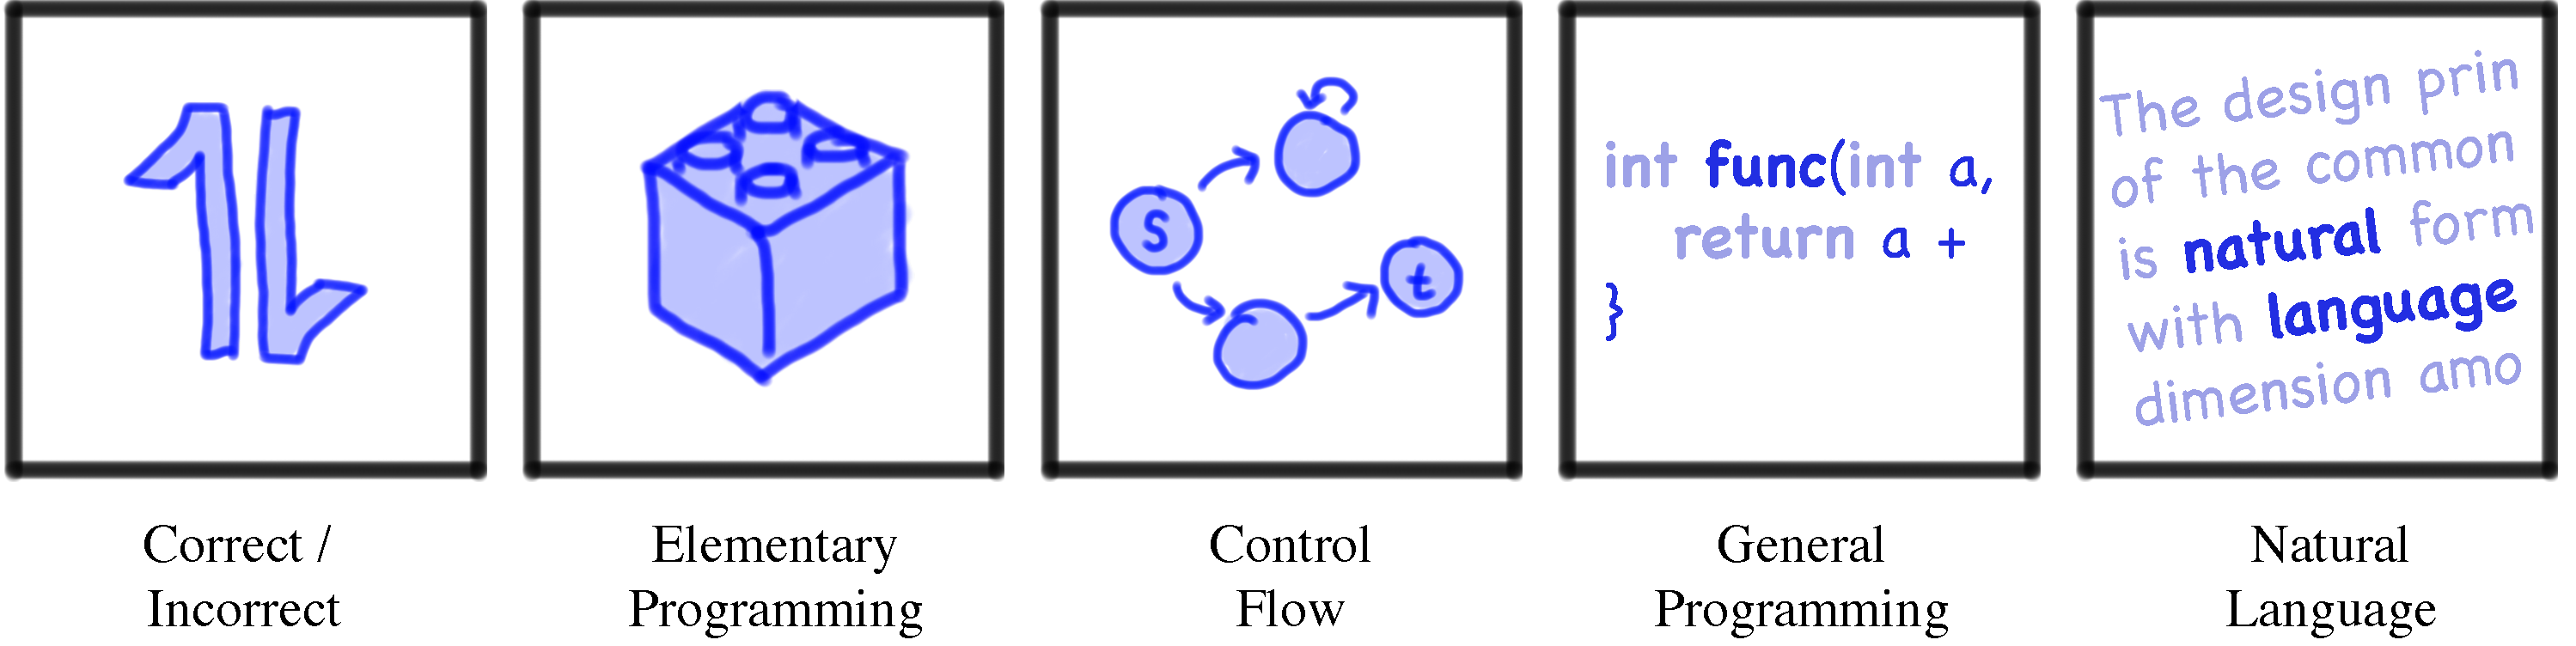
\includegraphics[width=1.0\textwidth]{img/assnType_all}
\caption[Assignment types]{
The different types of assignments covered in this thesis.
\label{fig:assnTypes}
}
\end{figure}

Specifically we identified the following different types of computer science assignments arranged in relative feedback complexity: 
\begin{enumerate}
\item Correct / Incorrect problems where students are asked either a multiple choice or short answer question and their response is coded as either being the right or wrong answer. 
\item Maze Programming assignments, which are designed for K-12 students and involve a simple maze which the students navigate using blocks that represent maze moves and may include standard control flow paradigms (like repeat, while and if)
\item Turing Complete Control Flow Programming assignments, in which students program in a language that is provably Turing complete, but does not involve user defied variables.
\item Functional Programing assignments, in which students program in a language that is turning complete and has user defined variables. We assume that programs are single threaded.
\item Natural Language assignments, in which students write up proposals and reports in English text.	
\end{enumerate}

This list is not exhaustive for all computer science assignment types. Of note, it does not include parallel programming assignments or problems from the theoretical branch of computer science. We collected at least one dataset for each of the different assignment types. See table \ref{tab:thesisDataTable} for details. 

\begin{table}[h]
 \centering
 \ra{1.3}
 \begin{tabular}{lp{1.8cm}p{1.8cm}p{1.8cm}p{1.8cm}p{1.8cm}}
   \toprule

   \tabhead{Statistic} & \tabhead{Khan \linebreak Geometry} & \tabhead{Code.org Academy} & \tabhead{Stanford CS106A} &  \tabhead{Coursera M.L.} & \tabhead{Coursera H.C.I.} \\

   \midrule

   Students & 1.0 $M$ & 1.2 $M$ & 2.7 $K$ & 26.1 $K$ & 7.2 $K$ \\
   Assignments  & 69 & 20 & 5 & 8 & 10 \\
   Submissions & 14.4 $M$ & 22.8 $M$ & 312.0 $K$ &  1.0 $M$  & 14.1 $K$ \\
   Type & Correct / Incorrect & Elementary Programs & Control Flow & Functional Programs & Natural Language \\
   Temporal & Yes & Yes & Yes & No & No \\

   \bottomrule
 \end{tabular}
 \caption[Summary of datasets]{Summary of datasets analyzed. $K = $ thousands and $M = $ millions. M.L. = Machine Learning and H.C.I = Human Computer Interaction }
 \label{tab:thesisDataTable}
\end{table}

When student work on programming assignments, we are parse their submissions into Abstract Syntax Trees (ASTs) and execute them on unit test inputs. We consider two submissions to be equal if their ASTs are identical. When possible, in addition to collecting the final submission that a student turns in for an assignment, we also collect the trajectory of partial solutions that they generate as they work their way from a blank project.

\section{Program Submission Sparsity}


An interesting observation that we made is that for every single programming assignment dataset that we analyze in this thesis, the frequency of submissions fits a Zipf's law distribution. 
\begin{figure}[ht]
\center
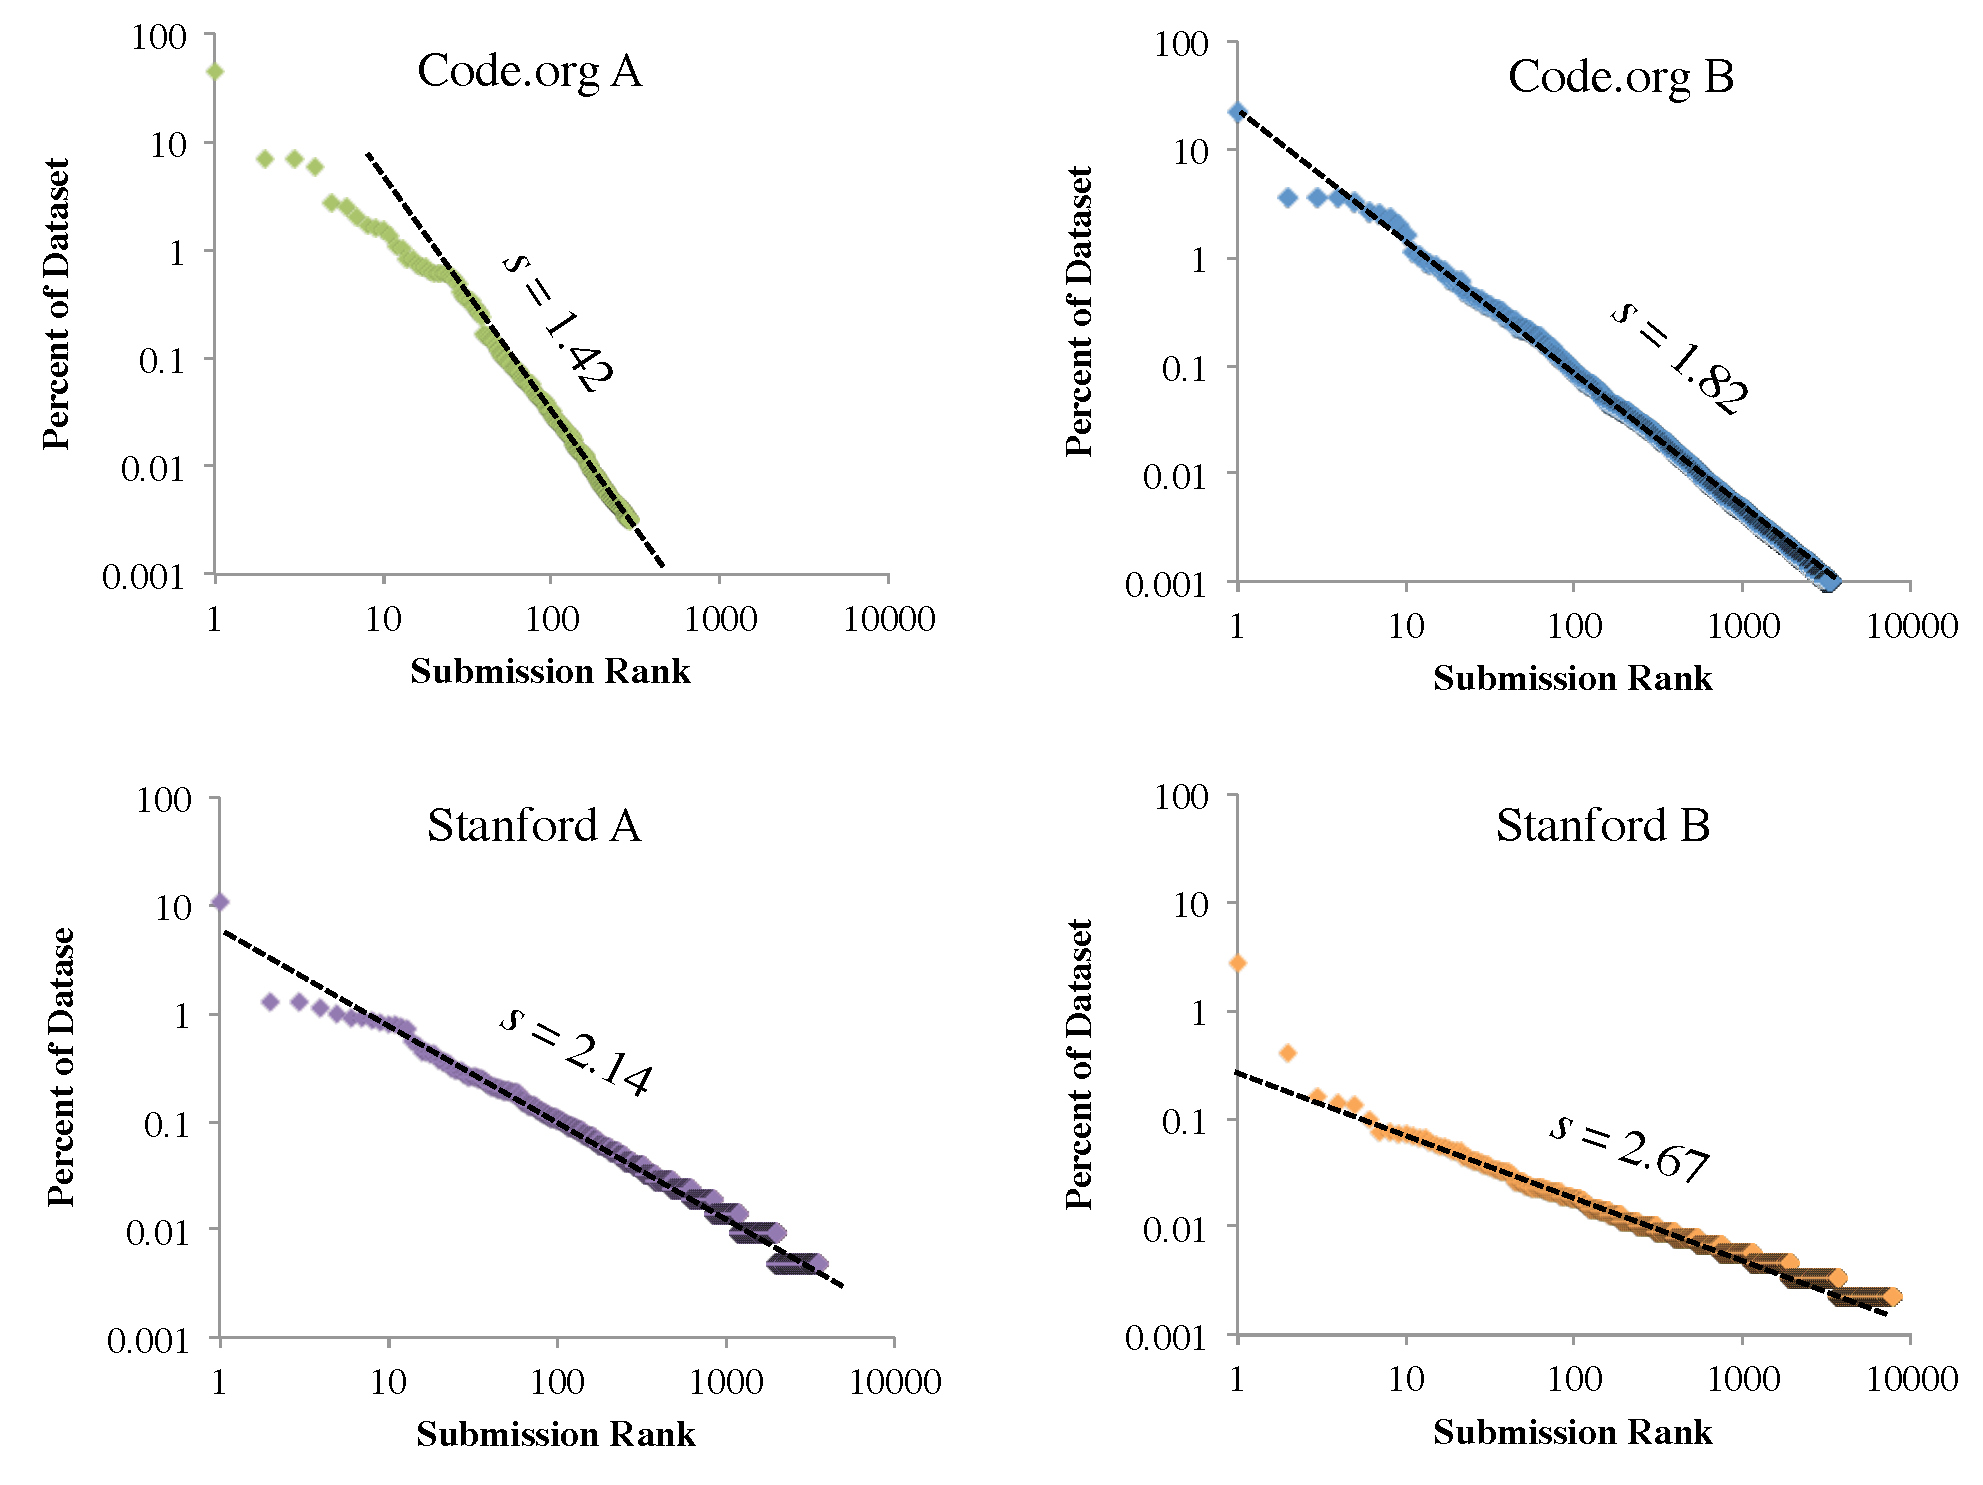
\includegraphics[width=1.0\textwidth]{img/zipfAll}
\caption[Submission Sparcity]{
Zipf plots for five assignments examined in this thesis. The designation of A and B assignments are used to differentiate different problems from the same platform. The $s$ value is the power parameter of a Zipf fit. All assignments have temporal data except for machine learning$^*$ and thus the $s$ parameter for that one assignment is not directly comparable to the others.
}
\label{fig:zipfAll}
\end{figure}
This is true for datasets where we have temporal data and datasets for which we only have final solutions. See figure \ref{fig:zipfAll}. Interestingly this trend even applies to the simplest programming assignment in the Code.org dataset where learners are only able to concatenate three commands -- and do not use any control flow elements. We have also noticed that the distribution of sub-programs also follows a Zipf's law distribution. The head of the distributions follow different patterns. The Zipf tendency seems to apply after the 10\ts{th} most common submission. Zipf law distributions often arise when data is generated in a hierarchical manner. Since students likely make a series of hierarchical decisions when solving a problem, and since programs are written in a way that produces hierarchical ASTs, it makes sense that the datasets are Zipfian. The implications are twofold. First, even for the most simple programming assignments that we look at there is a non-zero probability that a new submission will never be seen before and that will always be true regardless of how large a dataset we collect. The second implication is that we can use the exponent of the Zipf fit to compare the ``sparsity" of different programming assignments. This is particularly nice because the exponent is independent of the size of the dataset. Figure \ref{fig:zipfAll} shows the fit for all datasets for which we had temporal data. Sparsity can only be compared for datasets that were collected in a similar way (for example one cannot compare the Zipf fit for an assignment where we have all student partial solutions with one where we only have final solutions).

 An interesting observation is that the subjective ``complexity" ordering of assignment types that we chose matches the order of exponent parameters for the corresponding Zipf law distributions. This suggests one way to measure assignment complexity. Another observation is that the exponent of the Zipf distribution for the partial solutions to Stanford B is almost 3. This represents a very steep drop-off. For assignments that are more complex, the probability becomes increasingly small that one would ever observe two identical partial solutions.

\section{Approaches}

Our approach is to apply a disciplined machine learning paradigm to facilitate autonomous (or semi-autonomous) feedback at scale. Specifically we develop systems that try to capture emergent learner structures. 

\subsection{Big Picture First}

The problem of adding autonomy to the provision of feedback is hard. But the difficulty varies widely between different assignment complexities (and submission sparsity). In this dissertation we are going to start with the simplest and least sparse computer science assignments and work up in increasing levels of feedback difficulty focusing on the thematic split made in figure \cite{fig:assnTypes}. The largest difference that arises as complexity increases is that quickly program submissions become so sparse that it is hard to find temporal patterns in student work. Thus for the two simplest categories (Incorrect/Correct and Maze Programming Problems) we develop systems for autonomous feedback based on trajectories, which is a very rich source of information. However for the next two levels of complexity (Control Flow and Functional Programming) we have to first solve the problem of finding patterns in the space of submissions so that we can understand student trajectories in a more dense, latent space. One way to understand this is that we are marching down the different layers of emergent structure. The first question we ask is: can we understand students across a curriculum? Then for harder problems we ask, can we understand students as they work through a single question? For absolute hardest class of assignments, general programming tasks, we ask ourselves, can we understand how a single partial solution relates to others?

\subsection{Understand Students}

The ultimate goal of this line of research is to provide a scientific advance in our understanding of how to autonomously provide feedback to students. However there are unique challenges posed by the science of education. Three particularly notable challenges with regard to research on feedback is that (1) student experiments are expensive, (2) the mechanisms are complex so it is often hard to tease apart context or confounds and (3) learning outcomes are often multi-dimensional and long term.

It is ethical grey area to provide an experience for a student that is worse than what they would have otherwise received. There is a desire is similar to the, ``do no harm" Hippocratic oath taken in the field of medicine (where harm includes leaking any private student data). A clear example of this is that there is tremendous desire to never give feedback to students that is misleading. As a direct result experiments on live students are expensive. It is hard to convince an instructor to run a study and when a study is done it has to be performed under strict guidelines. Moreover, it is difficult to measure costs and benefits in an educational setting. Educational outcomes are multi-dimensional and involve short term and long term effects. An intervention may have broad effects on learners and testing those effects often is too invasive. Finally, even when an experiment is run on students and a reasonable education objective is selected and evaluated, it is still difficult to understand how different parts of a complicated feedback system should be attributed for observed results. As an example providing feedback often involves first autonomously understanding a student and then turning that understanding into English text that is presented to a student. It is difficult to tease the two apart.

You can think of giving feedback 
To overcome these challenges we focused on developing and testing systems that can understand students. In every chapter we identify a machine learning problem that can be used as the basis for autonomous feedback and can be directly evaluated with \emph{off-line} data. We will set out to solve these machine learning questions to the best of our ability. The task of then developing a human computer interaction system for optimally helping students is interesting and important, but outside the scope of this dissertation.

Aside: understanding can be measured either by predicting what s student will do, or by predicting what a teacher would tell a student.

\subsection{Easy to Author}

The autonomous feedback engine must be easy to author so that new activities and inspired ideas can be incorporated without much friction. Otherwise, using a machine learning system could prevent development of new assignments. There is an inherent balance between trying to maximize the quality of our feedback and to minimize teacher time. The general constraint that we held to was to keep teacher grading time the same as it would be in a traditional class of only a few dozen students.

\section{Novel Contribution}

\begin{figure}[t]
\center
   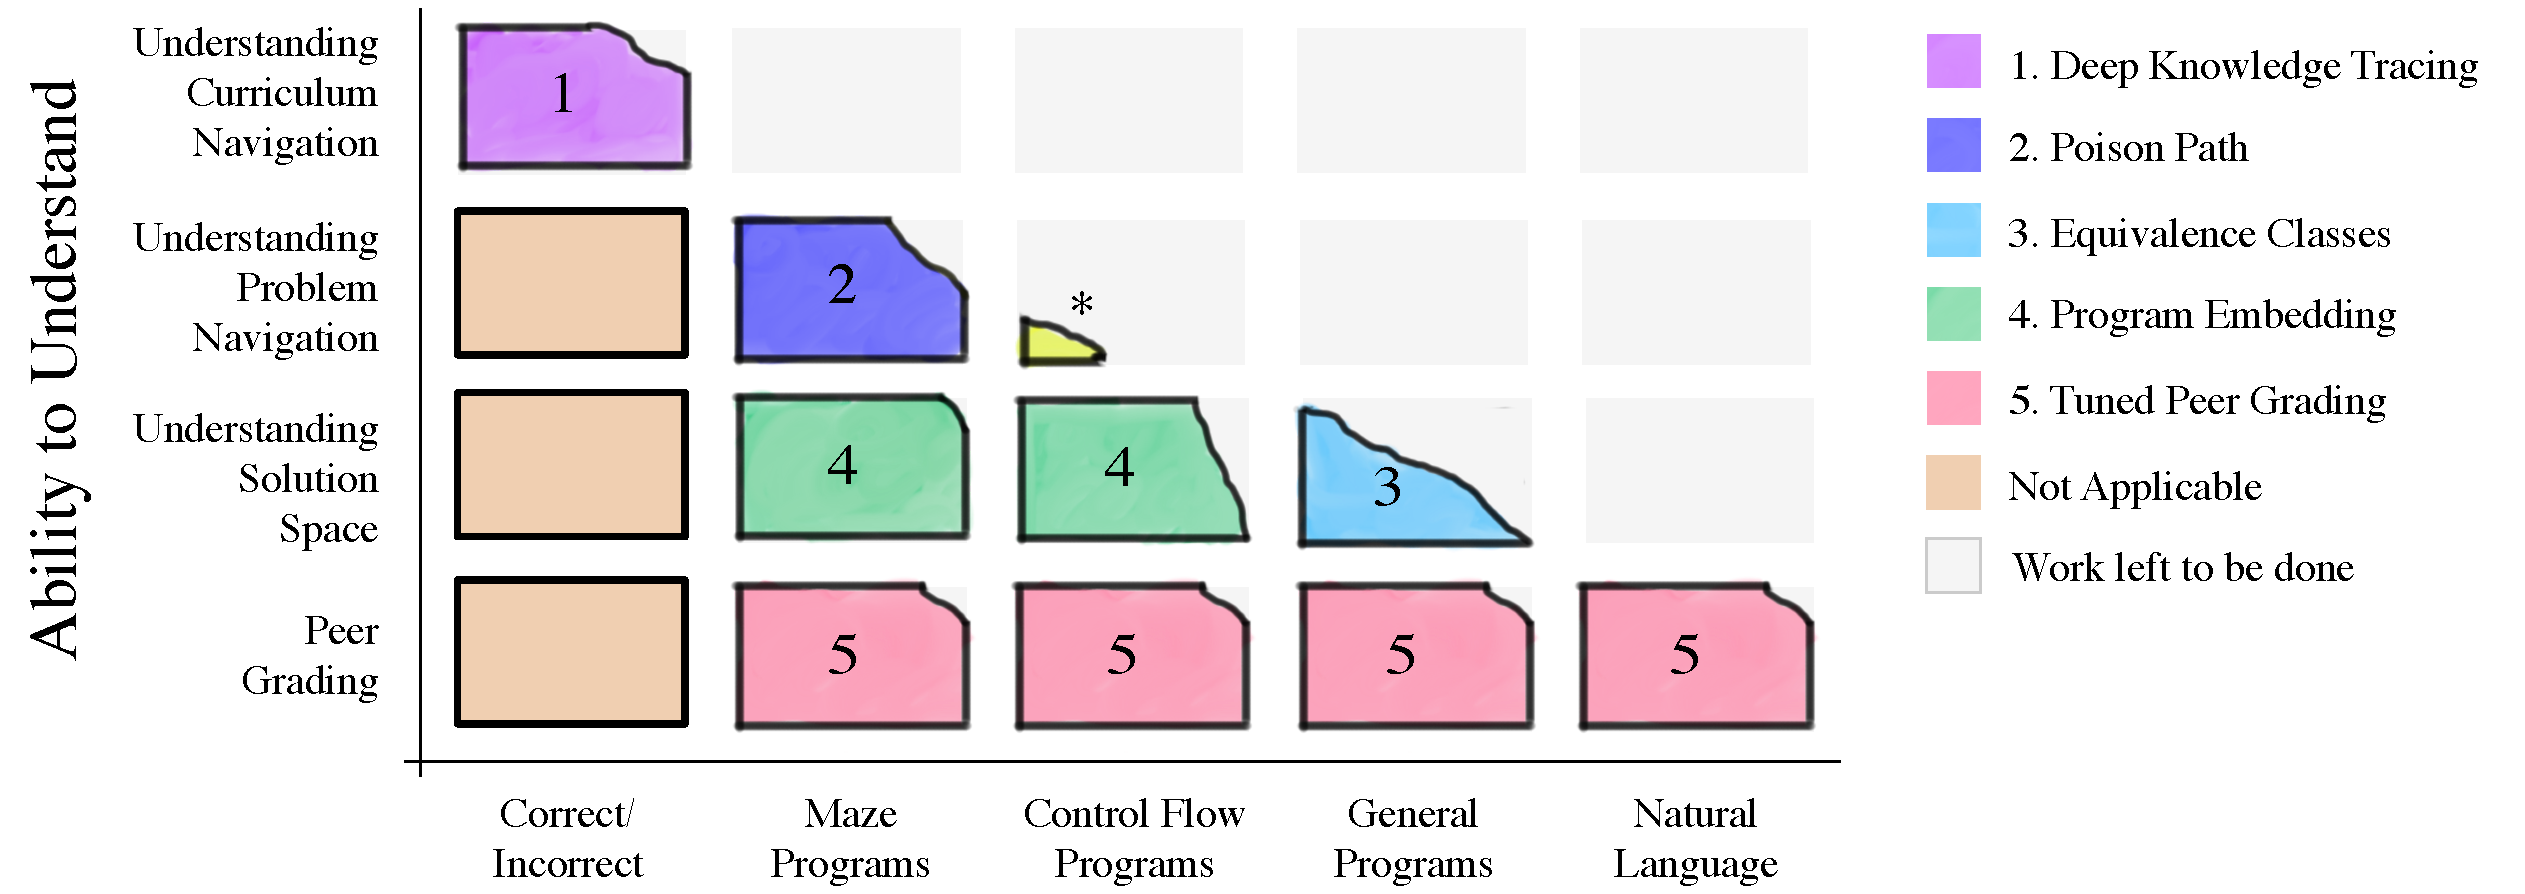
\includegraphics[width=1.0\textwidth]{img/intro-blocks.pdf}
\caption[Subjective contribution overview]{
Subjective measure of the degree to which different algorithms are able to understand students over the range of assignments that they apply.}
\label{fig:bigPicture}

\end{figure}

The challenge of how to provide autonomous feedback to students at scale remains an open problem. However I have made substantial progress towards understanding students as they learn. In each chapter we explore machine learning solutions to understanding increasingly more complex classes of assignments. 
In the first chapter we use recurrent neural networks to understand students as they solve correct/incorrect class of problems in Khan Academy. In the second chapter we find out what temporal patterns emerge when millions of students solve the same Code.org Maze assignments. In the third chapter we develop a neural network way to encode the functionality of control flow programming assignments. In the fourth chapter we present a way to autonomously discover equivalent sub-parts of general student programming assignments. Finally, in the fifth chapter we show how machine learning tools can be used to help in peer grading, the ubiquitous way to provide feedback online when autonomous methods are not available.

The most substantial contributions of this research are:
\begin{enumerate}
\item We achieved state of the art in knowledge tracing (and a 25\% increase of AUC on a standard dataset). 

\item Discovery of the Poison Path pattern in how students navigate solution spaces that both: predicts how teachers would suggest a learner make forward progress and has an almost perfect logrithmic relationship with the probability of a student succeeding in the future.

\item Two novel ways to simplify the solution space of programming assignments. A leading method to project program control flow functionality into euclidean space and an algorithm which can autonomously discover equivalent sub-parts of programs. Both means of simplifying solution expand the ability to propagate teacher feedback.

\item A novel way to `tune` the network of peer grades to simultaneously learn grading ability and assignment true scores (and a 33\% reduction in RMSE on an online design course).

\end{enumerate}
However, there are dozens of smaller corollaries that we arrived at as a result of our novel exploration of an unprecedented dataset. It is hard to quantify exactly where we stand with respect to autonomously providing feedback across the entire domain of programming assignments especially since the objectives we try to reach are slightly different for different problem types. However for each task I can subjectively express the degree to which the algorithms allow us to understand what students know. To do so I compose both (1) the degree to which a task reflects actionable understanding of a student and (2) the accuracy our algorithms were able to achieve on the task. As an example of the different utility of different prediction tasks: being able to predict exactly what a student will do represents a deeper understanding then being able to recognize that their last submissions was similar enough to another students that we can propagate feedback. For each of the new algorithms that we present I did my best to estimate algorithm ``understanding" over the range of assignments to which they are applicable. See figure \ref{fig:bigPicture}. While I have made substantial gains against the baselines of brute force annotation and propagation of feedback available from unit tests, there is still a substantial amount of room for improvement between the hull of our contemporary ability to understand students and the level that is possible.

The thesis is split into three parts. In the first part we explore how to understand students as they learn across curricula of simple answers. In the second part we will explore how to model student trajectories as they solve multi step programming tasks. In the third part we explore how to understand patterns in sparse student programs.

% include 
%One-on-one human tutoring can produce learning gains for the average student on the order of two standard deviations \cite{corbett2001cognitive}.



%\section{A Vision for the Future}
%Autonomous feedback from a system that understands learners as they navigate complex learning environments.
%In the far future, we may have powerful autonomous tutors. They will be able to understand what humans know and help them achieve learning goals in optimal ways. They will be free, or close to free. Their experience will persist. 

%The core emphasis is two solve two problems (1) Provide feedback, (2) Select appropraite material for students. 

%Achieving these milestones often involve sub-goals such as being able to predict what students will do, or how teachers would respond.

%The autonomous feedback engine must be easy to author so that new activities and inspired ideas can be incorporated without much friction.

%There are many different paths to an improved education landscape. This is just one interesting avenue.

%One reason that online is interesting is that it may enable scientific insights into learning

%Disiterata:
%Easy to author.
%Handle Richly Structured Activities


%Teachers have historically been faced with a difficult decision on how much personalized
%feedback to provide students on open-ended homework submissions
%such as mathematical proofs, computer programs or essays. On one hand, feedback
%is a cornerstone of the educational experience which enables students to
%learn from their mistakes. On the other hand, giving comments to each student
%can be an overwhelming time commitment. Hopefully autonomous feedback can be a powerful tool to help teachers of the future.

%In this work we present a set of approaches that are appropriate for different types of assignments. Ideally in the future we will be able to achieve the level of autonomous feedback we see for khan data for more complex assignments. 

%http://data.worldbank.org/indicator/SE.ENR.TERT.FM.ZS/countries/1W?display=graph